\section{Reducción de dimensionalidad}

\subsection{Introducción}
Como se mencionó previamente este ejercicio consistió en reducir la dimensión del
espacio original de los datos, la cual era de 850 componentes,
en un espacio de 9 componentes. El objetivo fue el de capturar las componentes
que mas explican la variabilidad de los datos en un espacio de dimensión menor.
Para esto se utilizaron redes neuronales entrenadas con los algoritmos de
\textit{Oja} y \textit{Sanger}. Al final del entrenamiento estos métodos terminan
habiendo modificado los pesos de la red de forma tal que su función asociada sea la de
proyectar el vector del espacio original en el subespacio de las primeras
componentes principales.

\subsection{Desarrollo}
La red neuronal que se utilizó para reducir dimensionalidad fué un perceptron
simple con función de activación lineal. Esta red contó con 850 neuronas de
entrada y 9 neuronas de salida. Esta topología fue pensada para poder clasificar
de forma no supervisada los documentos en 9 tipos de categorías.

Los algoritmo utilizados para el entrenamiento fueron los de \textit{Oja} y
\textit{Sanger} cuyos pseudocodigos se presentan a continuacion:
%%%%%%%%%%%%%%%%%%%%%% PONER PSEUDO DE OJA Y SANGER %%%%%%%%%%%%%%%%%%%%%%%%%%%%%

Se decidió separar el conjunto de datos en entrenamiento y testing con una
proporcion de 90\% y 10\% respectivamente. Los hiperparametros utilizados para
el entrenamiento de la red fueron $\eta = 0.0001$ y 500 epocas. La razon por la
que se decidió utilizar un coeficiente de entrenamiento de una magnitud tan
pequeña fue que los datos de entrada no estaban normalizados, logrando que
ocurran errores de overflow.

\subsection{Resultados}
Para una visualización mas clara de los datos se decidieron realizar tres
graficos diferentes en el que cada uno muestra de a tres componentes
principales. Se decidieron graficar los datos de testing con un marcador con
forma de triangulo para diferenciarlo de los circulos que representan los datos
de entrenamiento. Los resultados obtenidos se presentan a continuacion:


\begin{figure}[H]
  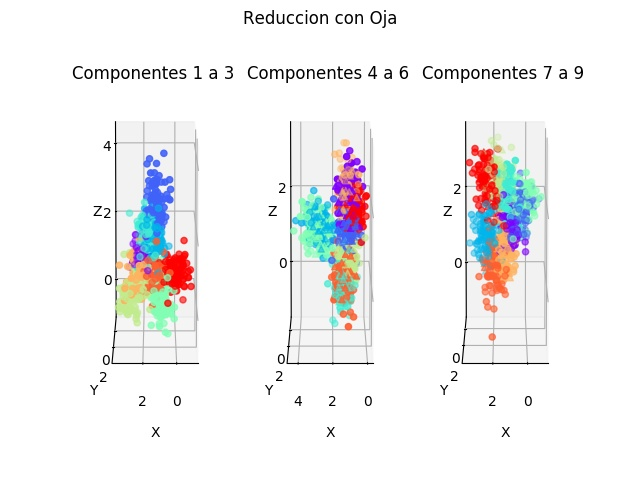
\includegraphics[width=160mm]{imagenes/reduccion_Oja_1.jpg}
  \caption{Vista desde arriba con Oja}
\end{figure}

\begin{figure}[H]
  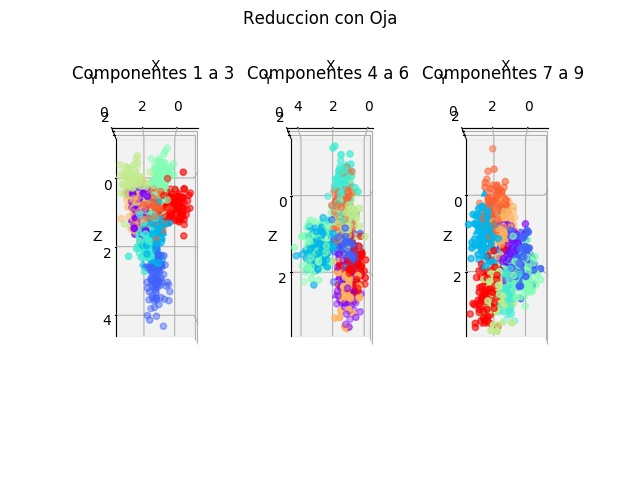
\includegraphics[width=160mm]{imagenes/reduccion_Oja_2.jpg}
  \caption{Vista desde abajo con Oja}
\end{figure}

\begin{figure}[H]
  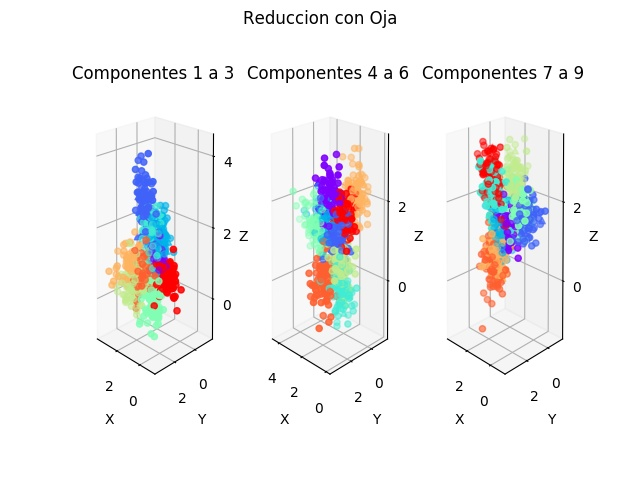
\includegraphics[width=160mm]{imagenes/reduccion_Oja_3.jpg}
  \caption{Vista de costado con Oja}
\end{figure}

\begin{figure}[H]
  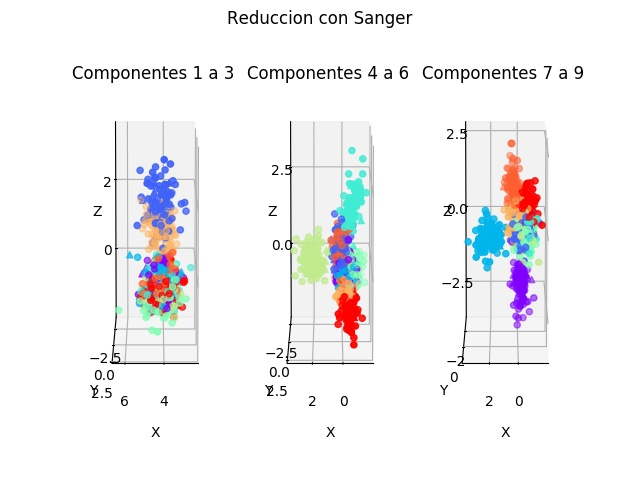
\includegraphics[width=160mm]{imagenes/reduccion_Sanger_1.jpg}
  \caption{Vista desde arriba con Sanger}
\end{figure}

\begin{figure}[H]
  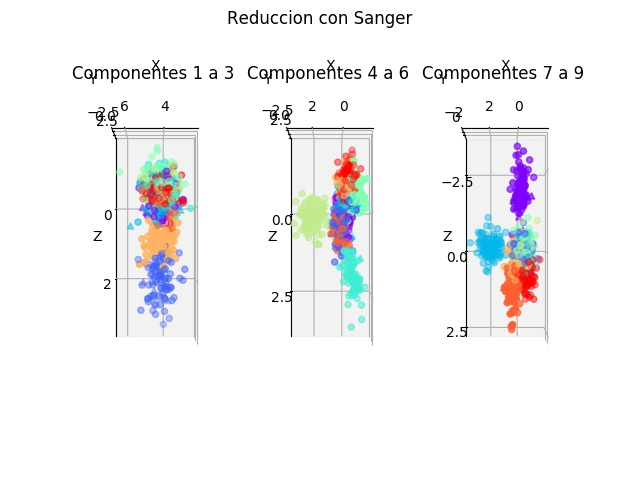
\includegraphics[width=160mm]{imagenes/reduccion_Sanger_2.jpg}
  \caption{Vista desde abajo con Sanger}
\end{figure}

\begin{figure}[H]
  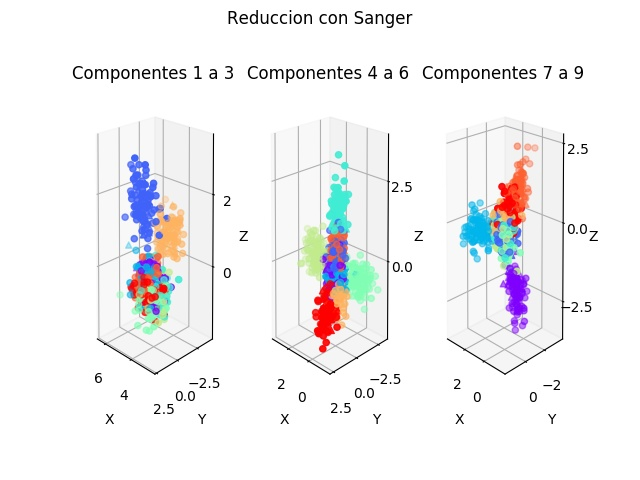
\includegraphics[width=160mm]{imagenes/reduccion_Sanger_3.jpg}
  \caption{Vista de costado con Sanger}
\end{figure}

Se observó que los vectores generados por el algoritmo de Sanger son mas descriptivos en comparacion a los generados por Oja.
 Es decir, que lograron una mejor separacion de los datos. Una posible justificación a este razonamiento es que los pesos generados
  por el algoritmo de Sanger convergen siempre al mismo vector, generando con ello siempre la misma proyeccion.

\subsection{Conclusión}
Como conclusión se pudo destacar que al tener los datos proyectados en las 9 componentes principales se pueden ver 9 clusters bien diferenciados espacialmente.
Esto logra la posibilidad de clasificar facilmente los documentos en 9 categorías distinas mediante la aplicacion de un clasificador como por ejemplo un perceptron multicapa.
Tambien se mejorararia los tiempos de entrenamiento ya que luego de ser preprocesada la entrada, los datos tienen una dimension menor y por lo tanto la entrada del clasificador
es mucho mas chica.

Estos modelos por si solos no sirven para clasificar, sino mas bien para darse una idea de cuantas clases hay dentro de los datos de entrada. Tambien sirven para preprocesar
 la entrada que luego será ingresada en un clasificador, conformando asi un modelo de tipo híbrido.
\newpage
